\documentclass{../../sheet}
\renewcommand{\logopath}{../../logos/}

\title{Einrichtungszeug}

\begin{document}
\maketitle

\aufgabe{WLAN - iOS und Android}
\begin{itemize}
  \item Im AppStore bzw. Playstore nach „geteduroam“ suchen und die App installieren
  \item Dann nach Universität Stuttgart suchen
  \item Nun Student wählen und eure Daten eingeben
  \item stxxxxxx@stud.uni-stuttgart.de - Benutzername und Passwort eingeben
  \item Nun auf Verbinden klicken und fertig
\end{itemize}

\aufgabe{WLAN - Windows}
\begin{itemize}
  \item Im Internet auf „geteduroam.app“ gehen und die Windows Version herunterladen
  \item Dann nach Universität Stuttgart suchen
  \item Nun Student wählen und eure Daten eingeben
  \item Nun auf Verbinden klicken und fertig
\end{itemize}

\aufgabe{WLAN - MacOS}
\begin{itemize}
  \item Im Internet auf „uni-stuttgart.de/eduroam“ gehen
  \item Gruppe „Student“ wählen
  \item Lädet das Konfigurationspaket herunter
  \item In euren Systemeinstellungen auf „Geräteverwaltung“ gehen
  \item Nun über das Plus-Symbol das Konfigurationspaket hinzufügen
  \item stxxxxx - Benutzername
  \item euer Passwort eingeben
  \item Nun auf Verbinden klicken und fertig
\end{itemize}
\newpage
\aufgabe{WLAN - Linux}
\begin{itemize}
  \item Im Internet auf „uni-stuttgart.de/eduroam“ gehen
  \item Als Benutzergruppe „Student“ wählen
  \item Unten links auf „einen anderen Installer auswählen“ klicken
  \item „Linux“ auswählen
  \item Über den Button das Pythonskript herunterladen
  \item Im Terminal mit \texttt{\$ python3 [Dateipfad zum Pythonskript]} ausführen.
  \item Den Anweisungen folgen und Benutzername (stxxxxxx@stud.uni-stuttgart.de) sowie Passwort eingeben
\end{itemize}

\newpage




\includegraphics[width=1\linewidth]{../img/memeIDE.jpg}

\aufgabe{Instalation - IntelliJ IDEA}


Geht auf „jetbrains.com/toolbox-app/“ und ladet die Toolbox herunter. \\
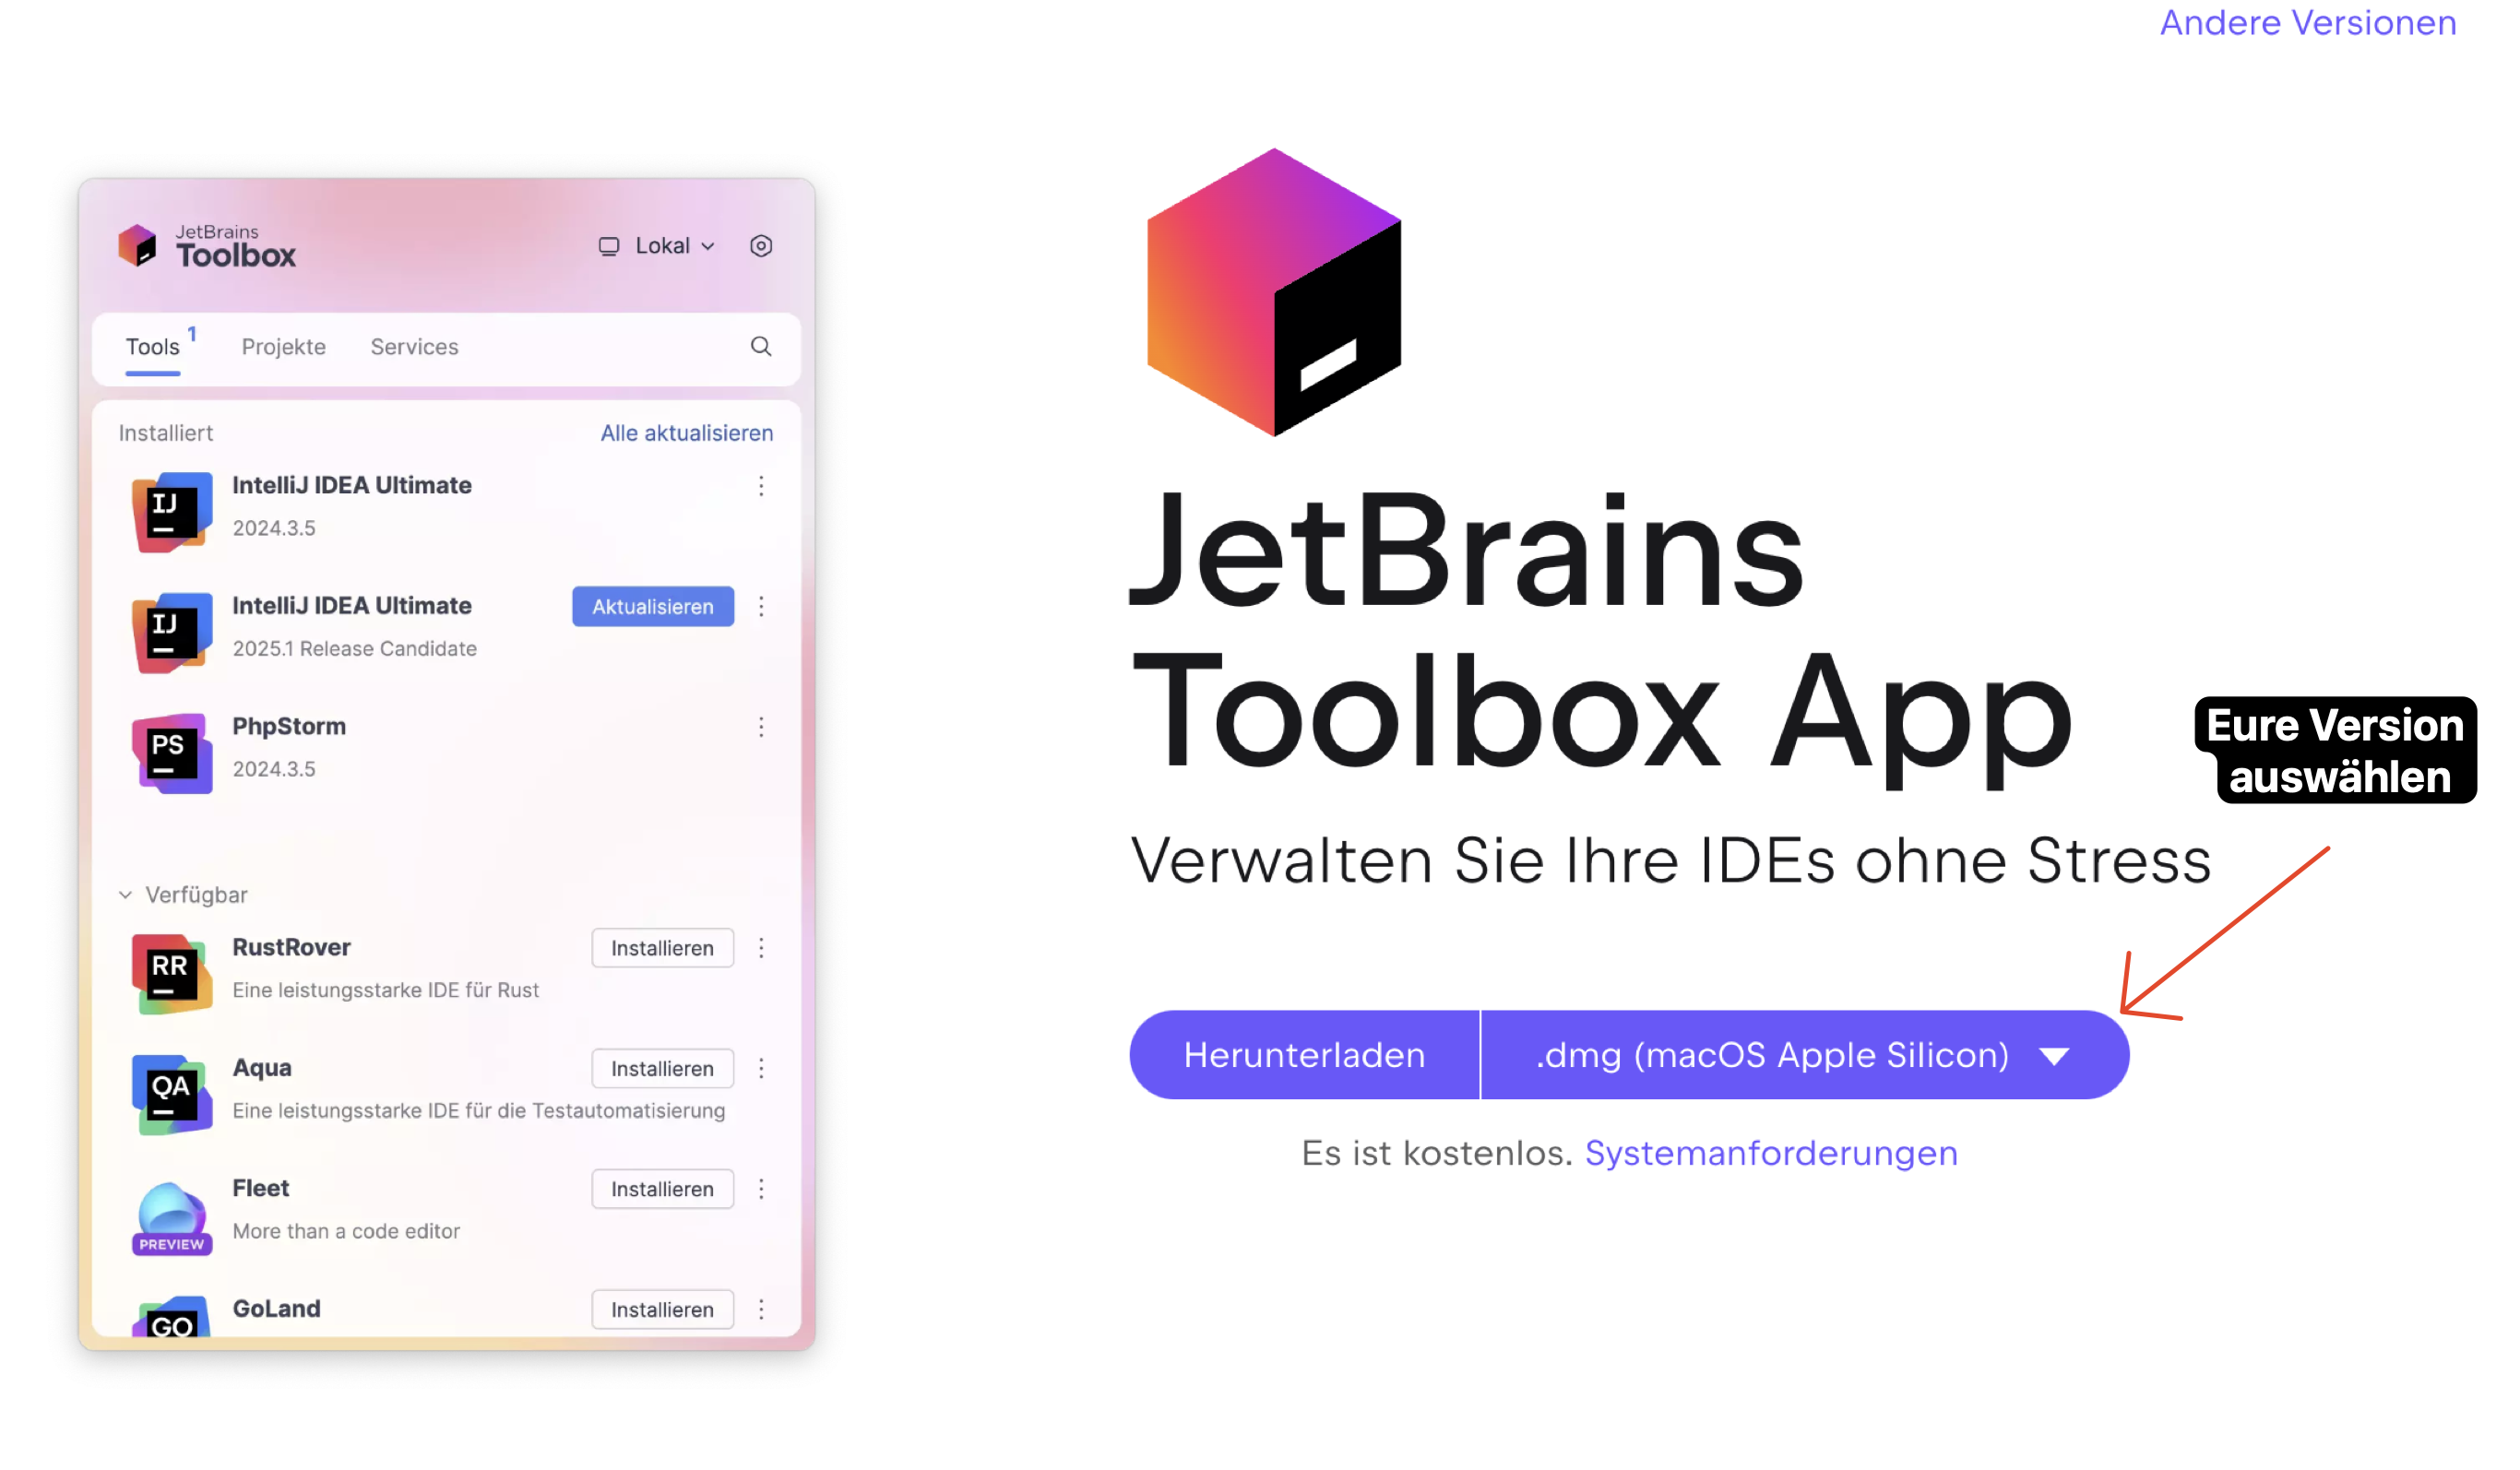
\includegraphics[width=1\linewidth]{../img/toolBoxDownload.png}

\newpage

Nach der Installation der Toolbox öffnet sich ein
Fenster. Wählt „IntelliJ IDEA
Community Edition“ aus und klickt auf „Install“.\\

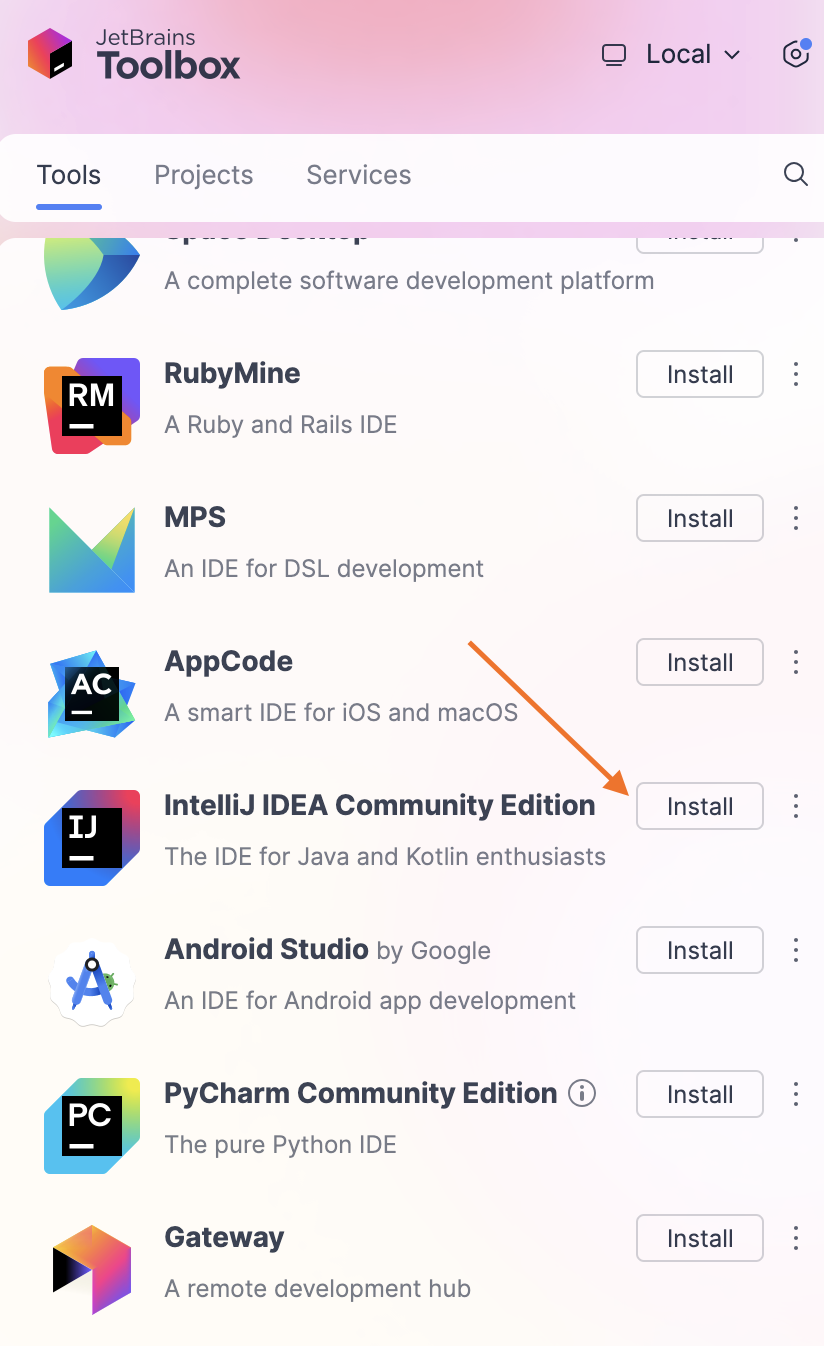
\includegraphics[width=0.5\linewidth]{../img/IntelliJDownload.png}

\newpage

\aufgabe{JDK - Installation}
Wir benötigen ein JDK (Java Development Kit), um Java Programme zu schreiben und
auszuführen.
\begin{itemize}
  \item IntelliJ öffnen
  \item MacOS: File/Datei gehen oben links in der Menüleiste
  \item Windows keine Ahnung
  \item Auf \texttt{Project Strucutre} klicken
  \item Dann auf \texttt{SDKs}
  \item Dann auf das + Symbol klicken und auf \texttt{Download JDK}
  \item OpenJDK Version 21 verwenden
  \item Microsoft OpenJDK als Anbieter/Vedor auswählen
  \item Speicherort auswählen (Standartpfad sollte reichen)
\end{itemize}

\newpage

\aufgabe{Projekt erstellen}
\begin{itemize}
  \item In IntelliJ auf neues Projekt erstellen/ New Project klicken
  \item Java auswählen und das Projekt firstProjekt nennen
  \item Nun nen geeigneten Speicher Ort auswählen Achtung: KEIN Git Reposotory erstellen
  \item Als Build System IntelliJ verwenden und als JDK unsere derzeitig herruntergeladene 21 auswählen
  \item Wir wollen keinen Sample Code
\end{itemize}

Es sollte nun so bei euch aussehen:

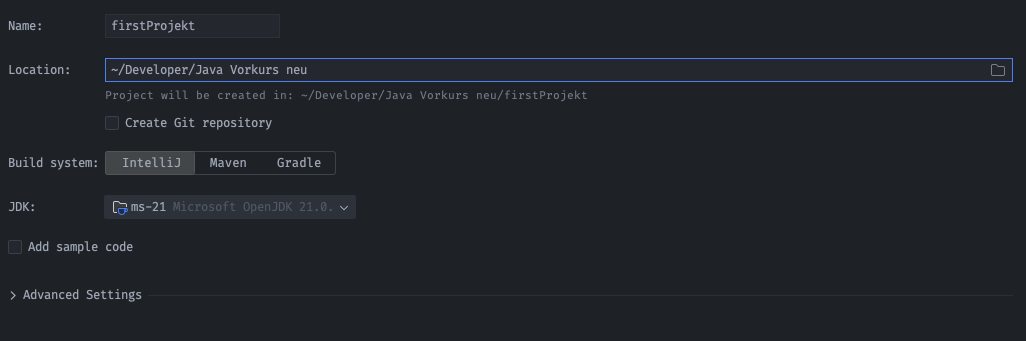
\includegraphics[width=1\linewidth]{../img/projektCreation.png}

\begin{itemize}
  \item Nun auf Create klicken und das Projekt wird erstellt
  \item Nun links in der Projektansicht auf src rechtsklicken und eine neue Java Klasse erstellen
  \item Diese Klasse Main nennen und auf Enter drücken
  \item Nun sollte sich eine neue Datei öffnen, in der wir unseren Code schreiben
\end{itemize}

\aufgabe{Erste Java Klasse}
Nun schreiben wir folgenen Code in die Main Klasse rein
\begin{minted}[fontsize=\Large]{java}
    public class Main {
      public static void main(String[] args) {
        System.out.println("Hallo Welt!");
      }
    }
  \end{minted}


\end{document}